%\documentclass [12pt]{article}
%\usepackage{hyperref}
%\usepackage{fullpage}
%\usepackage{graphicx}

% !TEX root = QuickStart.tex

%\begin{document}

%\maketitle

%\vspace{4in}

%\includegraphics[clip=on,width=\columnwidth,height=0.8\textheight,keepaspectratio]{logo2.png}

%\pagebreak

\section{Veusz Cookbook}
\label{sec:VeuszCookbook}

Most of the plots in this Guide were created with Jeremy Sanders' Veusz plotting package.
Veusz is an open-source and runs on Windows, Mac OS X,
and Linux. Veusz can be downloaded from \url{https://veusz.github.io/}. What follows are a few recipes for basic Cloudy plotting tasks that will get you started with Veusz. For more information, see the Veusz manual at \url{https://veusz.github.io/help-support/}. 
This document assumes that you are using Veusz 1.6 or later.

\subsection{Steps to Import data}

There is an important distinction in this step.
If you create an ``unlinked data set'' Veusz will make your data part of the
Veusz plot file. 
This is good if you want a single self-contained file.
If you create a ``linked data set'' the plot will be linked to the original
data file.  If you update the data file the plot will be updated with no further work.

Veusz does not read spreadsheet files directly.
If you work with your data in a spreadsheet you should save the
data in a field-delimited format.
CSV (comma separated values) or tabs are good choices.

\textbf{Heads up:} Data files created by Cloudy have a first line with 
column headings for the data that follow. These headings have spaces and 
special characters (/, + , -, {\_}, etc.). If you encounter problems with 
Veusz not being able to open files with unlinked data sets, removing 
these characters from your data and re-importing may fix the problem.

\begin{enumerate}
\item Click ``Data''
\item Select ``Import''
\item Choose the file that contains your data clicking ``Browse'' and selecting the file
\item If the data is delimited, select the ``CSV'' tab.
\item Under the ``File Preview'' box select the correct delimiter
\item At the bottom, you have the option to link the dataset to the original file.
\item Click ``Import'' and each column of your data will be saved in a dataset designated by the column heading.
\item Click ``Close''
\end{enumerate}

\subsection{Steps to plot your data (XY points)}

\begin{enumerate}
\item Click ``Insert''
\item Select ``Add xy'' : xy1 will be created in the top white box on the left (Editing Box)
\item The middle box (properties box) on the left side gives the properties of the xy1 pointset
\item In the properties box, click the blue down arrow to the right of ``X data''
\item Select the dataset that you want to appear on the x-axis
\item Repeat steps 4 and 5 for the ``Y data''
\end{enumerate}

\subsection{Steps to Export Plot to PDF}

\begin{enumerate}
\item Click ``File''
\item Select ``Export''
\item Choose the file location with the ``where'' drop down.
\item Click the blue down arrow to the right of the ``Files of Type'' (at the bottom)
\item Choose ``Portable Document Format (*.pdf)''
\item Choose the destination and file name then click ``Save''
\end{enumerate}

\subsection{Change From Points and Line (default) to Line only}

\begin{enumerate}
\item With the desired pointset selected in the Editing Box, select the ``Main'' tab in the Formatting Box (bottom on the left).
\item Click the blue down arrow on the ``Marker'' drop down box
\item Select ``none''
\end{enumerate}

\subsection{Add x-axis title:}

\begin{enumerate}
\item Select ``X'' (of the ``axis'' type) in the Editing Box
\item Enter the desired title for the x-axis in the ``Label'' textbox inside the Properties Box
\end{enumerate}

\subsection{Add y-axis title:}

\begin{enumerate}
\item Select ``Y'' (of the ``axis'' type) in the Editing Box
\item Enter the desired title for the y-axis in the ``Label'' textbox inside the Properties Box
\end{enumerate}

\subsection{Add a second plot:}

\begin{enumerate}
\item Repeat the Steps to plot your data (XY points)
\end{enumerate}

\subsection{Change Line Properties:}

\begin{enumerate}
\item Select the desired pointset in the Editing Box
\item Click the second tab called ``Plot line'' in the Formatting Box
\item In this tab one can change the color, width, style, and transparency of the line for the selected pointset.
\end{enumerate}

\subsection{Adding a Key or Legend:}

\begin{enumerate}
\item Click ``Insert''
\item Select ``Add Key'' -- This will create a blank key/legend box that can be dragged and dropped.
\item Select a pointset from the Editing Box
\item In the Properties Box, enter the text to appear in the key/legend box in the textbox called ``Key text''
\end{enumerate}

\subsection{Create a 2D dataset (Needed for contour or image graphs):}

\begin{enumerate}
\item Ensure that your individual data columns are already imported
\item Click ``Data''
\item Select ``Create 2D''
\item Type in a name for your 2D dataset in the ``Name'' textbox
\item Ensure that the middle option, ``From x, y, and z {\ldots}'', is selected in the ``Method of Creating Dataset'' Box.
\item In the ``Values'' section, choose the desired x, y, and z individual datasets
\item Click ``Create'' -- It should tell you that the dataset was created at the bottom of the form.
\item Click ``Close''
\end{enumerate}
	
\subsection{Create a Contour Plot:}

\begin{enumerate}
\item Click ``Insert''
\item Select ``Add contour''
\item In the Properties Box, select the desired 2D dataset
\end{enumerate}

Veusz automatically chooses contours. It is possible to change the number of 
contours by changing the ``Number Levels'' property. Changing the 
``Scaling'' property changes the way that the contour levels are chosen. 
If the contours are chose automatically, it is important to
specify the ``min'' and ``max'' contours.

\subsection{Set Contour Levels Manually:}

\begin{enumerate}
\item Ensure that the desired contour set is selected in the Editing Box.
\item In the Properties Box, change the ``Scaling'' property to ``Manual''
\item Enter the desired contour levels in the ``Manual Levels'' textbox separated by commas.
\end{enumerate}

\subsection{Add contour labels:}

\begin{enumerate}
\item Click on the 2$^{nd}$ tab in the Formatting Box, called ``Contour labels''
\item Uncheck the ``Hide'' checkbox
\item The font, color, and size can also be adjusted here
\end{enumerate}

\subsection{A bit about contour plots:}

With a contour pointset selected, the Formatting Box contains 5 tabs. The 
first tab, called ``Main formatting'', only allows you to hide the contours.
The next tab over is called ``Contour Labels''. 
Here you can adjust the numerical labels for the contours.

The third tab from the left is called ``Contour Lines''. By default, there is one line style. 
This means that all of the contour lines will have the properties set by this line style. 
The ``Add''button will add a new line style to the list. With 2 line styles, 
the top line style will be applied to the lowest contour line. The second line style 
will be applied to the next lowest contour. The next contour line will then 
take the properties of the top line style. Each successive contour line will 
continue to cycle between the two available line styles. The ``Delete'' 
button deletes the lowest line style on the list. The checkbox to the right 
of the line style properties hides the contour lines that are described by 
the given line style.

The fourth tab is called ``Contour Fill''. It works just like the ``Contour Lines'' tab except
that it fills in the contour areas with different fillers (e.g. solid, vertical lines, etc.). It is also possible
to adjust the color of the fillers.

The fifth tab is ``Sub-contour Lines''. This tab allows you to add a specific number of contour sections evenly spaced between the defined
contour lines. The number of sections to add in between each defined contour line is set by the ``Levels'' textbox. The number of sub-contour lines that will appear between each defined contour is the number in the ``Levels'' textbox minus one. The ``Line Style'' section
of this tab works the same way as the ``Contour Lines'' and ``Contour Fill'' tab. Note that you have to uncheck the ``Hide'' checkbox to view
the sub-contours.

\subsection{Filled contour maps}

A variety of filled contour maps are available.  
Do insert / image and then select a 2D dataset.
Several color and grey-scales are available.

If you want both the contour lines and the filled image then the contours must be
on top of the filled contour.  

Figure \ref{fig:grid_extreme} shows an example, 
taken from the \cdCommand{grid\_extreme} test in the slow test suite.
This uses the spectrum2 colormap and goes from red to blue as the
temperature goes from low to high values.

\begin{figure}
\begin{center}
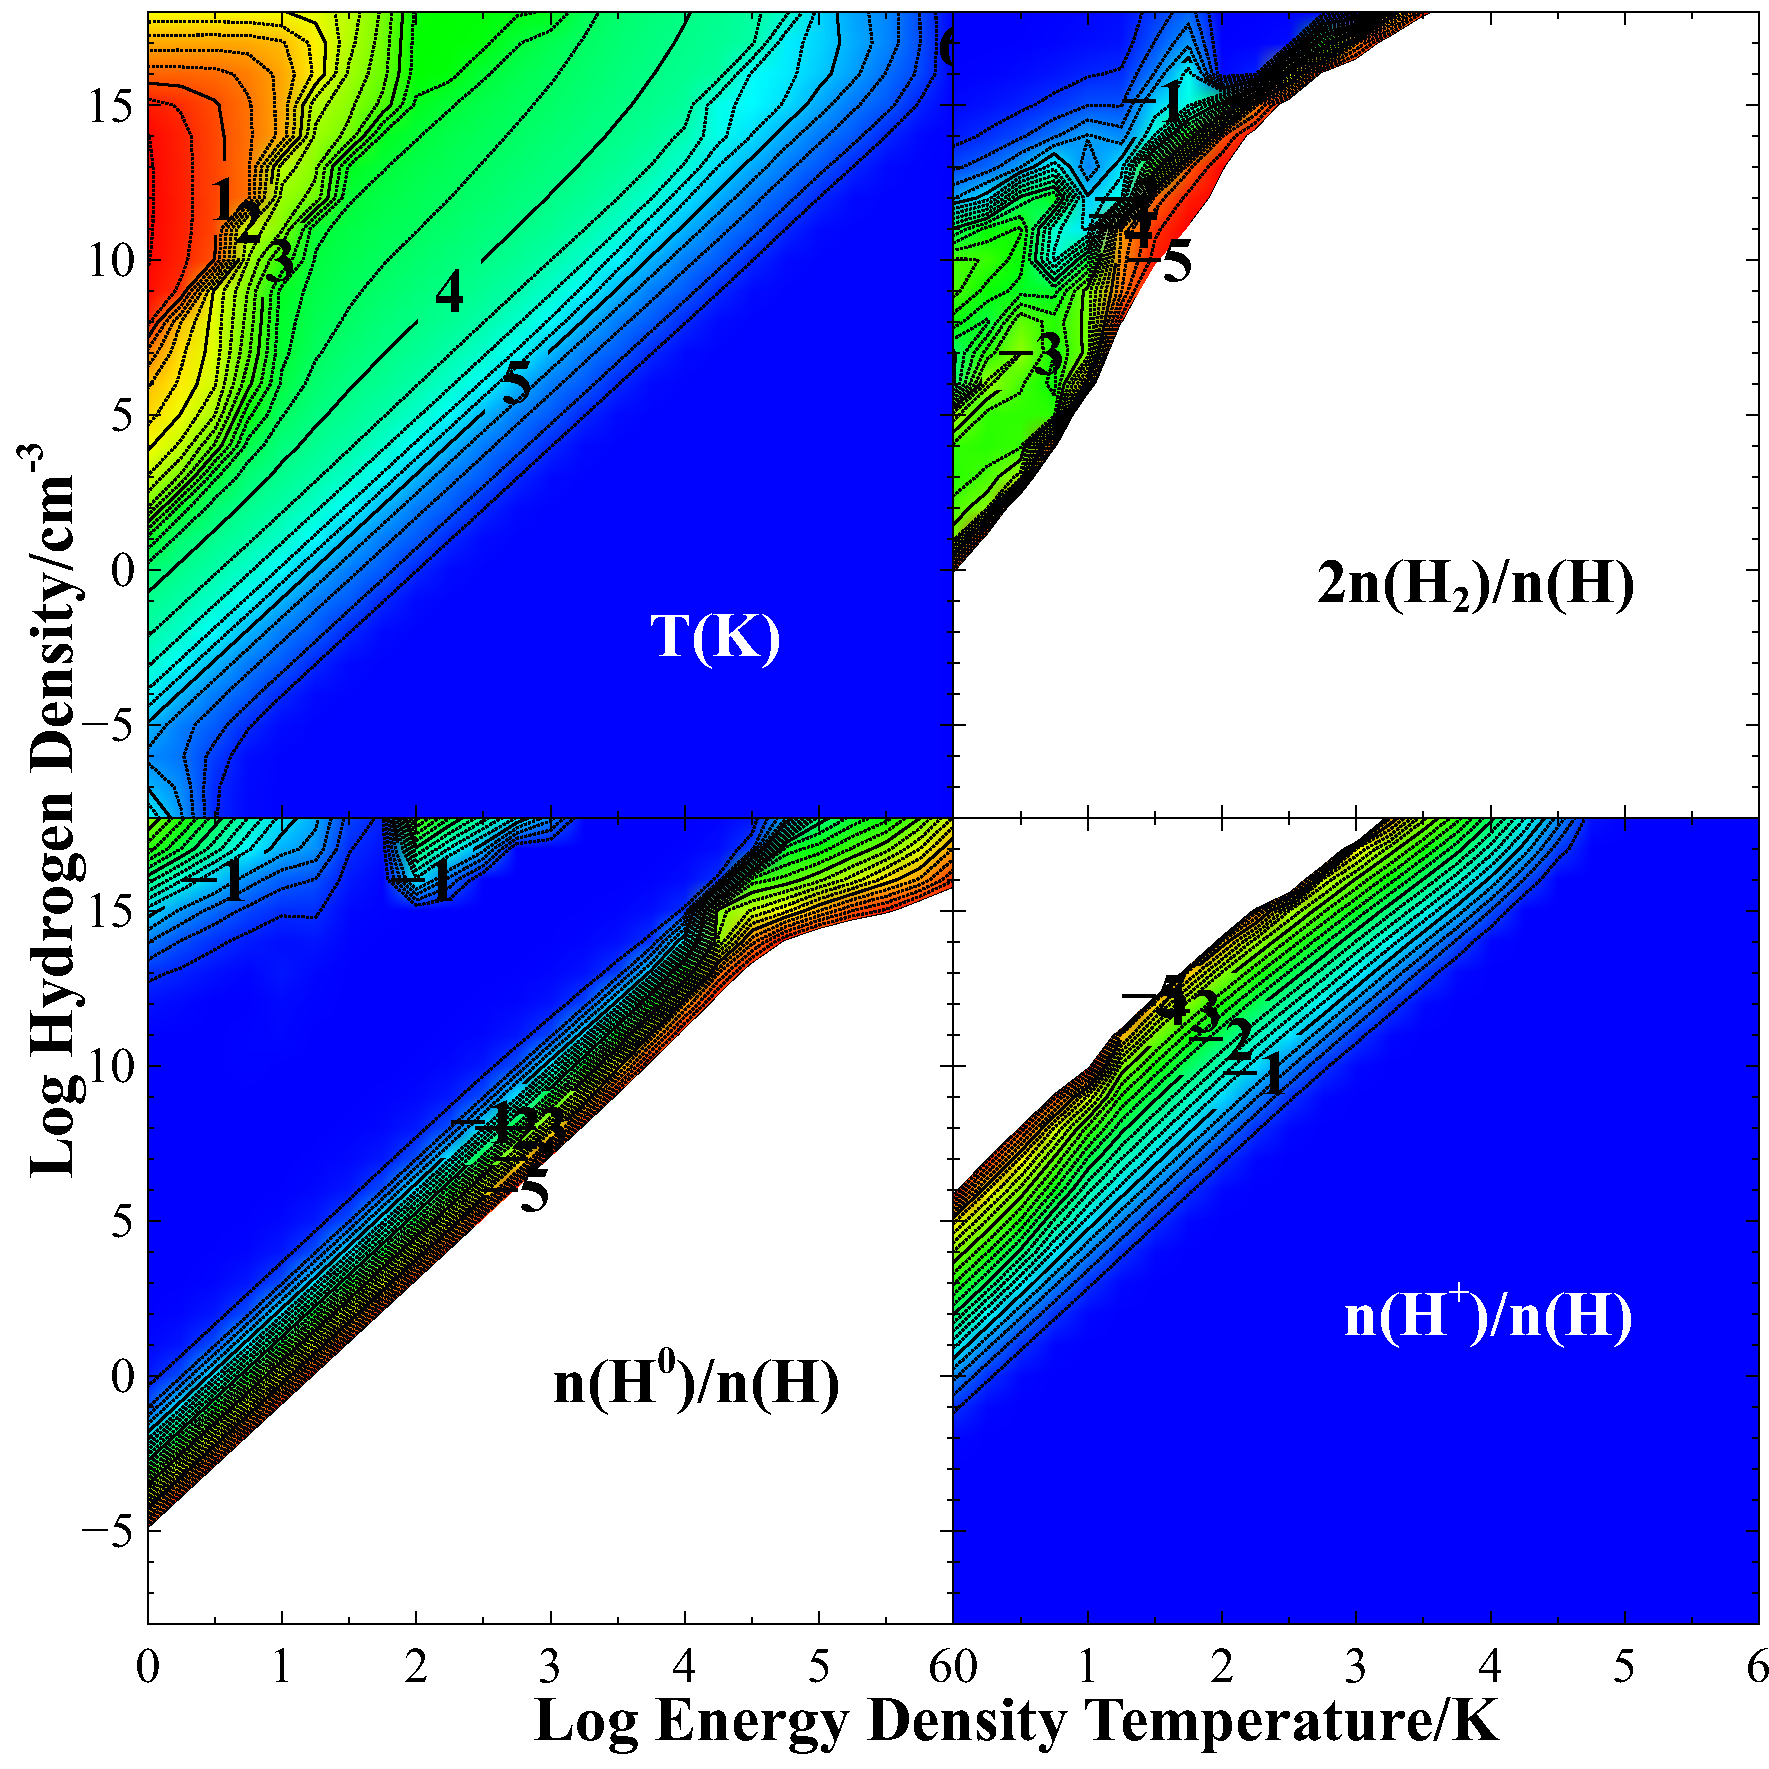
\includegraphics[clip=on,width=0.9\columnwidth,height=0.7\textheight,keepaspectratio]{grid_extreme}
\end{center}
\caption{This shows physical conditions over a very broad range of hydrogen density 
and energy-density temperature.  
The log of the electron kinetic temperature is shown in the upper left,
and hydrogen ionization and molecular fractions in the remaining panels.
The gas goes to the Compton temperature in the 
upper left corner of each panel, is in the blackbody limit across the top, and is close to LTE 
across the right-hand edges of the figure.}
\label{fig:grid_extreme}
\end{figure}

\subsection{Multiple graphs}

The graphs are made out of widgets that can be placed inside each other, e.g. 
graphs can be placed in pages, and different types of plotting widgets, e.g. xy or function, 
can be placed in graphs. 
You can also place graphs within a grid widget to get an arrangement of separate graphs.

Figure \ref{fig:orion_hii_pdr_pp} shows an example, 
taken from the Orion HII region / PDR simulation, of a nested plot.

\begin{figure}
\begin{center}
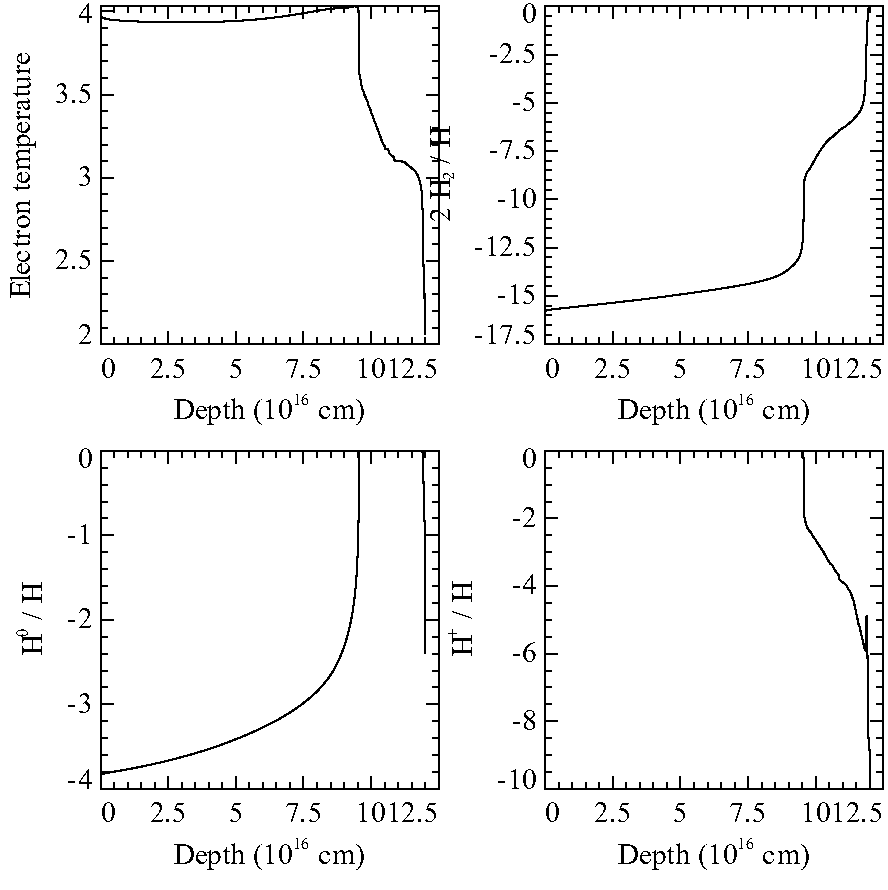
\includegraphics[clip=on,width=0.8\columnwidth,height=0.8\textheight,keepaspectratio]{orion_hii_pdr_pp}
\end{center}
\caption{The electron kinetic temperature, and fractions of H in H$_2$,
H$^0$, and H$^+$, are shown as a function of depth into the 
Orion H II region / PDR.}
\label{fig:orion_hii_pdr_pp}
\end{figure}

%\end{document}
